\chapter{Реализация индексов и статистика}
\section{Реализация индексов}
\subsection{Кучи}

Куча — это довольно простая структура. Данные в куче не имеют никакой
логической организации. Куча — это просто набор страниц и экстентов. 

SQL Server отслеживает, какие страницы и экстенты принадлежат объекту, с помощью специальных системных страниц, называемых страницами карты распределения индекса (Index Allocation Map, IAM). Каждая таблица или индекс имеет по
крайней мере одну страницу IAM, называемую первой страницей IAM. Одна страница IAM может указывать примерно на 4 Гбайт пространства. Страницы IAM объекта организованы в двунаправленный список. SQL Server хранит указатели на первые страницы
IAM в собственных внутренних системных таблицах. 


Следующий запрос извлекает основную информацию о таблице dbo.TestStructure.

\begin{lstlisting}[label=lst:funcReturn, language=sql]
	CREATE TABLE dbo.TestStructure
	( id INT NOT NULL,
	 filler1 CHAR(36) NOT NULL,
	 filler2 CHAR(216) NOT NULL );

	SELECT OBJECT_NAME(object_id) AS table_name, name AS index_name, type, type_desc
	FROM sys.indexes
	WHERE object_id = OBJECT_ID(N'dbo.TestStructure', N'U'); 
\end{lstlisting}

Столбец type хранит значение 0 для куч, 1 для кластеризованных таблиц (индексов) и 2 для некластеризованных индексов.

Можно узнать, сколько страниц выделено под объект, из функции динамического управления sys.dm\_db\_index\_physical\_stats или с помощью системной процедуры dbo.sp\_spaceused.

\begin{lstlisting}[label=lst:funcReturn, language=sql]
	SELECT index_type_desc, page_count,
		record_count, avg_page_space_used_in_percent
   	FROM sys.dm_db_index_physical_stats
		(DB_ID(N'tempdb'), OBJECT_ID(N'dbo.TestStructure'), NULL, NULL , 'DETAILED');
   	EXEC dbo.sp_spaceused @objname = N'dbo.TestStructure', @updateusage = true;
\end{lstlisting}

Обратите внимание на последний столбец первого запроса, avg\_space\_used\_in\_percent. Этот столбец показывает внутреннюю фрагментацию. Внутренняя фрагментация означает, что страницы не заполнены.

\subsection{Кластеризованные индексы}

\begin{figure}[h!]
	\begin{center}
		
\includegraphics[width=0.9\textwidth]{img/advice41.png}
	\end{center}
	\captionsetup{justification=centering}
\end{figure}



Основную информацию об индексе можно получить, запросив функцию динамического управления sys.dm\_db\_index\_physical\_stats. Следующий фрагмент кода будет использоваться в этой части занятия много раз, поэтому в дальнейшем будем называть его кодом <<проверки выделения кластеризованного индекса>>. 

\begin{lstlisting}[label=lst:funcReturn, language=sql]
	SELECT index_type_desc, index_depth, index_level, page_count,
		record_count, avg_page_space_used_in_percent
   	FROM sys.dm_db_index_physical_stats
		(DB_ID(N'tempdb'), OBJECT_ID(N'dbo.TestStructure'),
	NULL, NULL, 'DETAILED'); 
\end{lstlisting}


От фрагментации можно избавиться, если перестроить или реорганизовать индекс.
Реорганизация индекса — процесс более медленный, но менее ресурсоемкий.
В общем случае, следует выполнять реорганизацию индекса, если внешняя фрагментация менее 30\%, и перестраивать его, если она больше 30\%. Следующий код перестраивает индекс. 

\begin{lstlisting}[label=lst:funcReturn, language=sql]
	ALTER INDEX idx_cl_filler1 ON dbo.TestStructure REBUILD;
\end{lstlisting}

\begin{figure}[h!]
	\begin{center}
		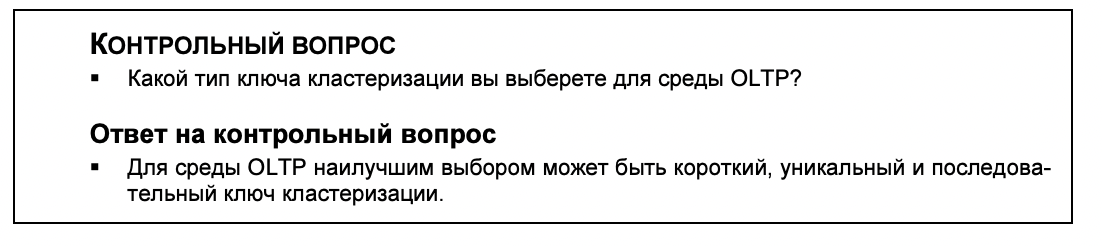
\includegraphics[width=0.9\textwidth]{img/control42.png}
	\end{center}
	\captionsetup{justification=centering}
\end{figure}


\subsection{Реализация некластеризованных индексов}

Операция извлечения строки из кучи называется уточняющим
запросом RID. Если запрос очень избирательный и ищет одну строку или
только небольшое количество строк, тогда индексный поиск с помощью
уточняющего запроса RID очень эффективен.


Если таблица организована как сбалансированное дерево, тогда указателем строк
является ключ кластеризации. Это означает, что когда SQL Server ищет строку, он
должен пройти все уровни на некластеризованном индексе, а затем также
все уровни кластеризованного индекса. Эта операция называется поиском
ключа.


В SQL Server 2012 существует способ хранения некластеризованных индексов.
Кроме стандартного хранилища строк, SQL Server 2012 может сохранять данные
индекса столбец за столбцом в так называемом индексе columnstore. Индексы columnstore могут многократно ускорить запросы хранилища данных, от
10 до 100 раз.


\subsection{Реализация индексированных представлений}


\begin{lstlisting}[label=lst:funcReturn, language=sql]
	CREATE VIEW Sales.QuantityByCountry
	WITH SCHEMABINDING
	AS
	SELECT O.shipcountry, SUM(OD.qty) AS total_ordered,
	 COUNT_BIG(*) AS number_of_rows
	FROM Sales.OrderDetails AS OD
	 INNER JOIN Sales.Orders AS O
	 ON OD.orderid = O.orderid
	GROUP BY O.shipcountry;
	GO
	CREATE UNIQUE CLUSTERED INDEX idx_cl_shipcountry
	ON Sales.QuantityByCountry(shipcountry);
	GO
\end{lstlisting}

\subsection*{Резюме занятия}
\begin{itemize}
	\item Можно сохранить таблицу как кучу или как сбалансированное дерево. Если таблица сохранена как сбалансированное дерево, она является кластеризованной; она также называется кластеризованным индексом.
	\item Можно создать некластеризованный индекс на куче или на кластеризованной
	таблице. 
	\item Также можно индексировать представление. 
\end{itemize}

\subsection*{Закрепление материала}

\begin{figure}[h!]
	\begin{center}
		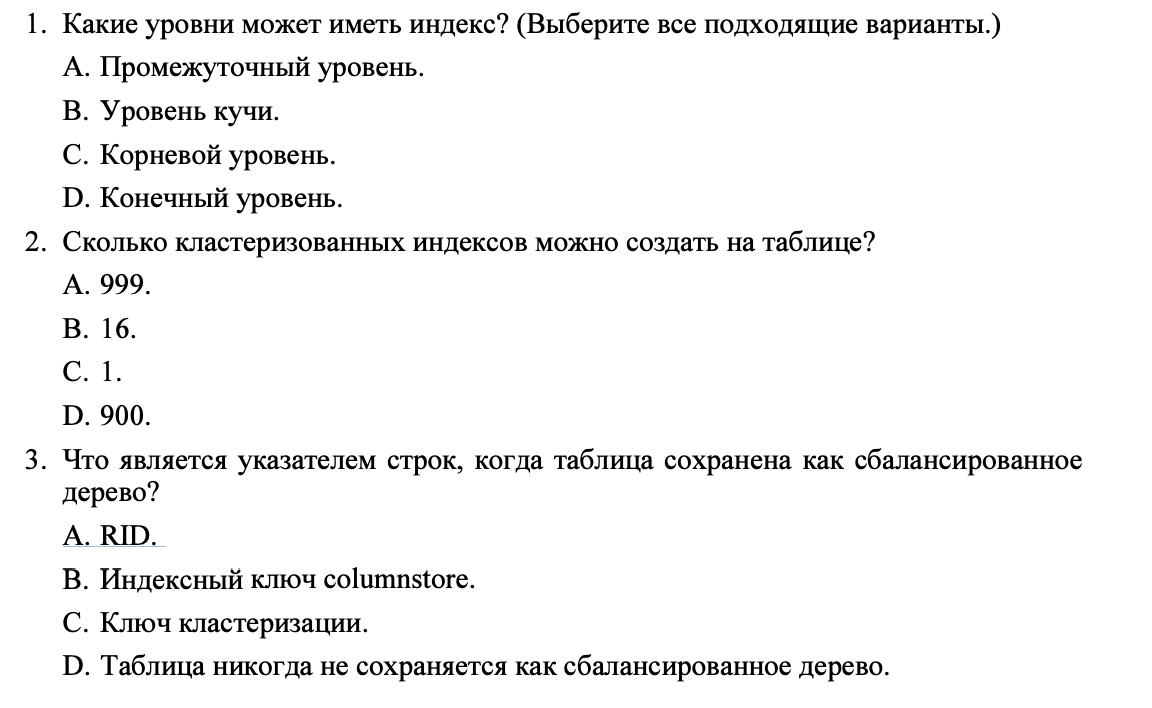
\includegraphics[width=0.7\textwidth]{img/zakrep43.png}
	\end{center}
	\captionsetup{justification=centering}
\end{figure}
\newpage

\subsection*{Ответы}

\begin{figure}[h!]
	\begin{center}
		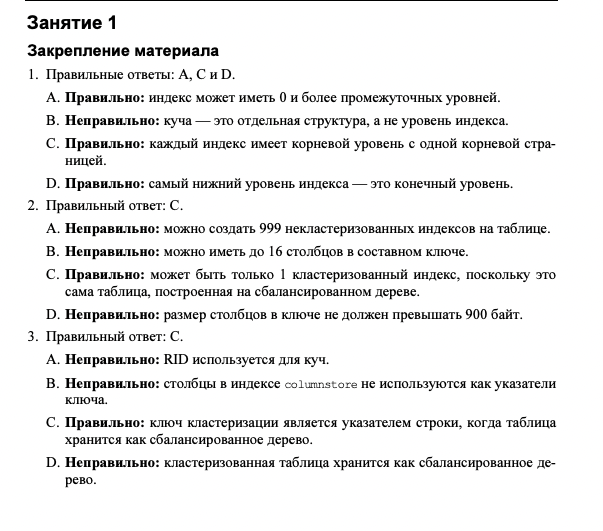
\includegraphics[width=0.6\textwidth]{img/ans43.png}
	\end{center}
	\captionsetup{justification=centering}
\end{figure}
\clearpage



\section{Использование аргументов поиска}

\subsection{Аргументы поиска}

Чтобы написать подходящий аргумент поиска SARG, вы должны быть уверены,
что столбец, имеющий индекс, появляется в предикате отдельно, а не как параметр
функции. Аргумент поиска SARG должен принимать форму столбца inclusive\_operator <value> или столбца <value> inclusive\_operator. Имя столбца должно стоять отдельно на одной стороне выражения, а константа или вычисляемое значение — появляться на другой стороне. В качестве операторов могут использоваться операторы =, >, <, =>, <=, BETWEEN и LIKE. Но оператор LIKE можно использовать, только если подстановочные символы \% или \_ не стоят в начале строковой переменной, с которой сравнивается столбец. 

\begin{figure}[h!]
	\begin{center}
		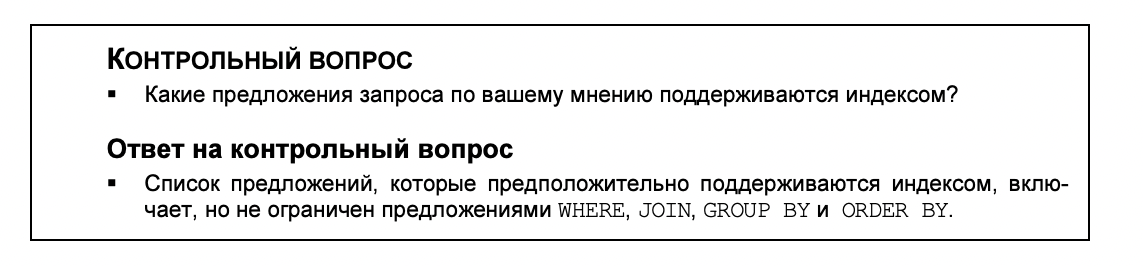
\includegraphics[width=0.9\textwidth]{img/control43.png}
	\end{center}
	\captionsetup{justification=centering}
\end{figure}

\subsection*{Резюме занятия}
\begin{itemize}
	\item Разные части запроса могут поддерживаться индексами.
	\item Следует рассматривать возможность использования предложений запроса WHERE,
	JOIN, GROUP BY, ORDER BY и SELECT с надлежащими индексами. 
	\item Следует писать подходящие аргументы поиска, не включая в выражения столбцы ключей индексов. 
\end{itemize}


\subsection*{Закрепление материала}

\begin{figure}[h!]
	\begin{center}
		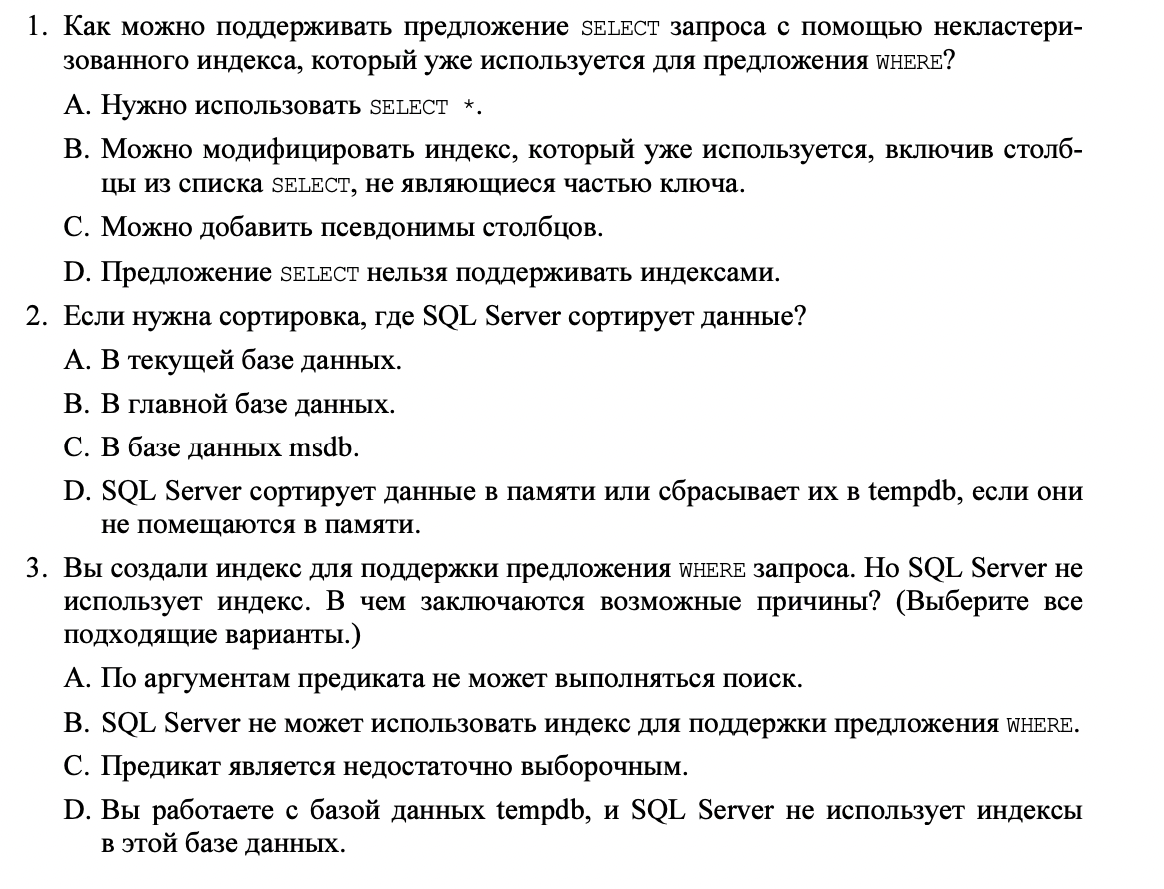
\includegraphics[width=0.9\textwidth]{img/zakrep44.png}
	\end{center}
	\captionsetup{justification=centering}
\end{figure}
\clearpage	

\subsection*{Ответы}

\begin{figure}[h!]
	\begin{center}
		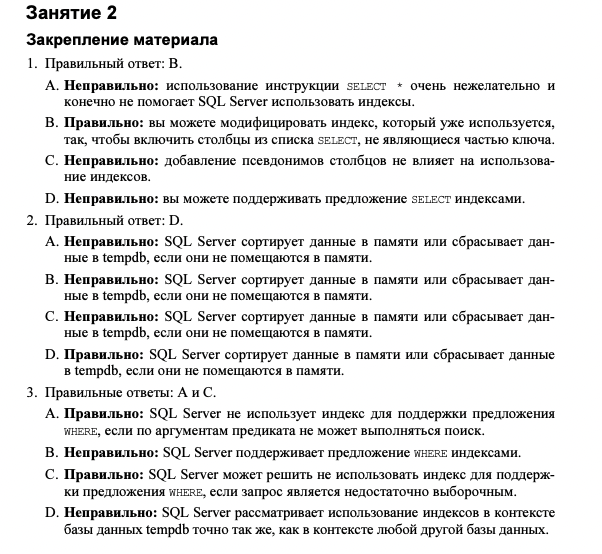
\includegraphics[width=0.9\textwidth]{img/ans44.png}
	\end{center}
	\captionsetup{justification=centering}
\end{figure}



\section{Основные понятия статистики}


\subsection{Автоматически создаваемая статистика}

Существуют три параметра баз данных, оказывающие
влияние на автоматическое создание статистики. 

\begin{itemize}
	\item AUTO\_CREATE\_STATISTICS. Когда этот параметр включен, SQL Server создает статистику автоматически.
	\item AUTO\_UPDATE\_STATISTICS. Когда этот параметр включен, SQL Server может автоматически обновлять статистику при достаточном количестве изменений в базовых таблицах и индексах.
	\item AUTO\_UPDATE\_STATISTICS\_ASYNC. Этот параметр определяет, использует ли SQL Server синхронное или асинхронное обновление статистики, во время оптимизации запроса.
\end{itemize}



\subsection*{Резюме занятия}
\begin{itemize}
	\item Оптимизатор запросов SQL Server использует статистику для определения количества элементов в запросе.
	\item Кроме предоставления права поддержки автоматической статистики SQL Server,
	можно также поддерживать статистику вручную. 
\end{itemize}


\subsection*{Закрепление материала}

\begin{figure}[h!]
	\begin{center}
		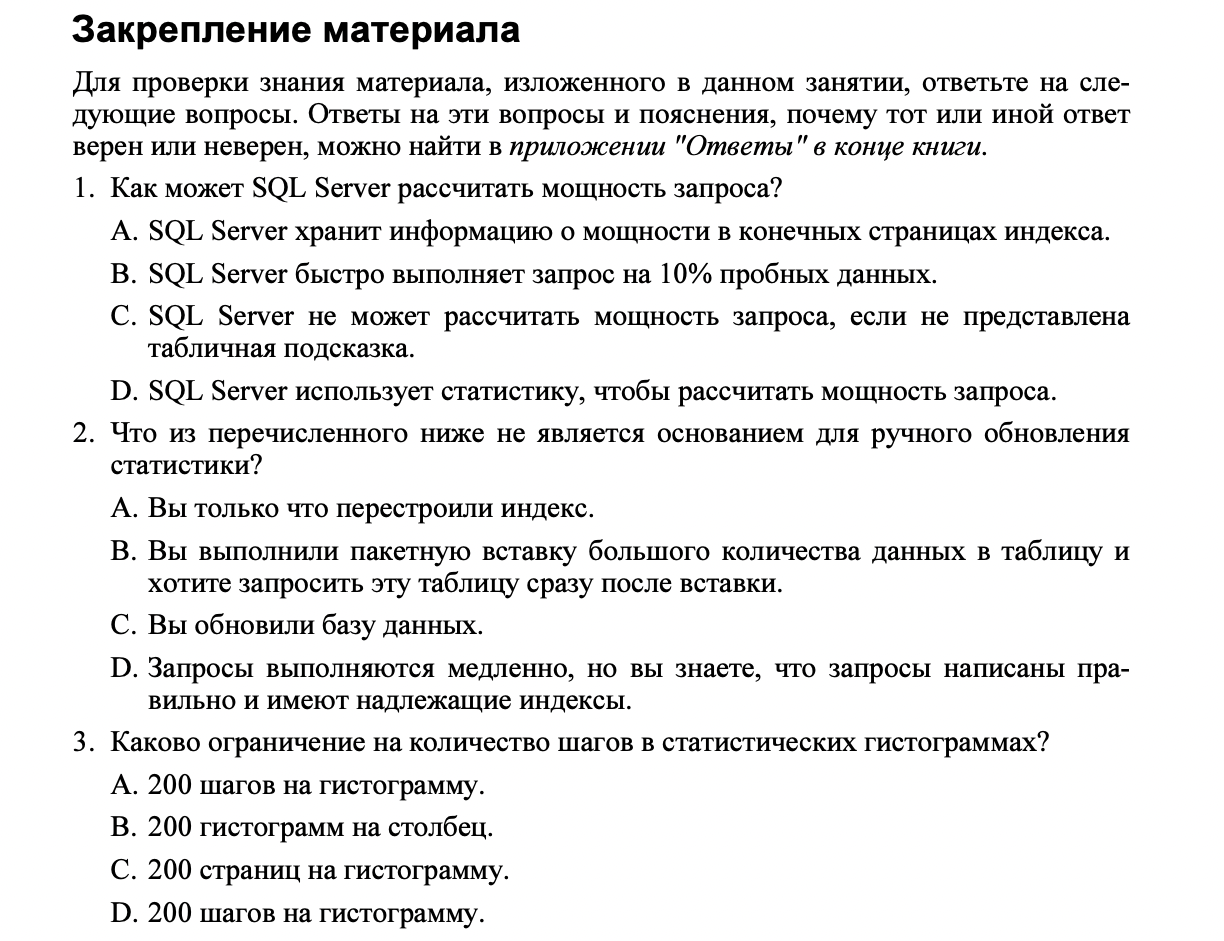
\includegraphics[width=0.7\textwidth]{img/zakrep45.png}
	\end{center}
	\captionsetup{justification=centering}
\end{figure}
\clearpage

\subsection*{Ответы}

\begin{figure}[h!]
	\begin{center}
		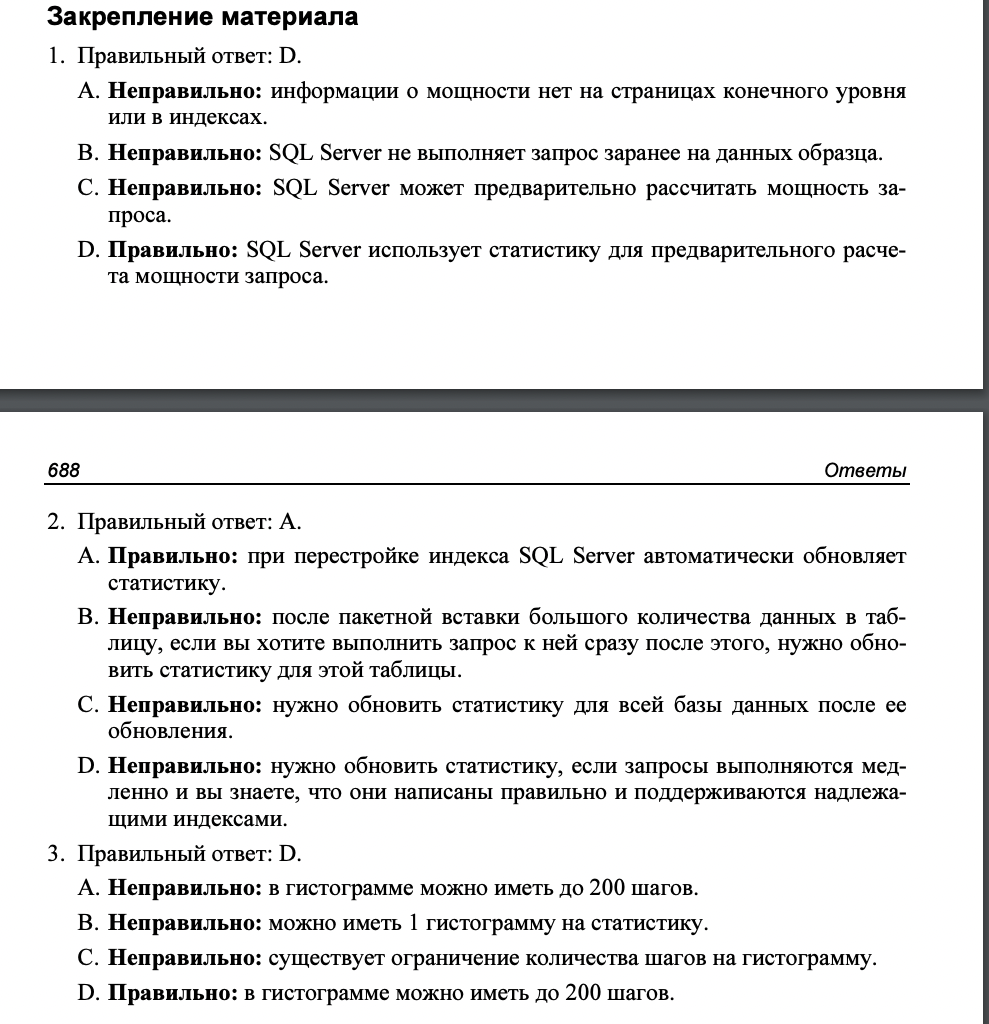
\includegraphics[width=0.9\textwidth]{img/ans45.png}
	\end{center}
	\captionsetup{justification=centering}
\end{figure}


\newpage
\subsection*{Упражнения}

\begin{figure}[h!]
	\begin{center}
		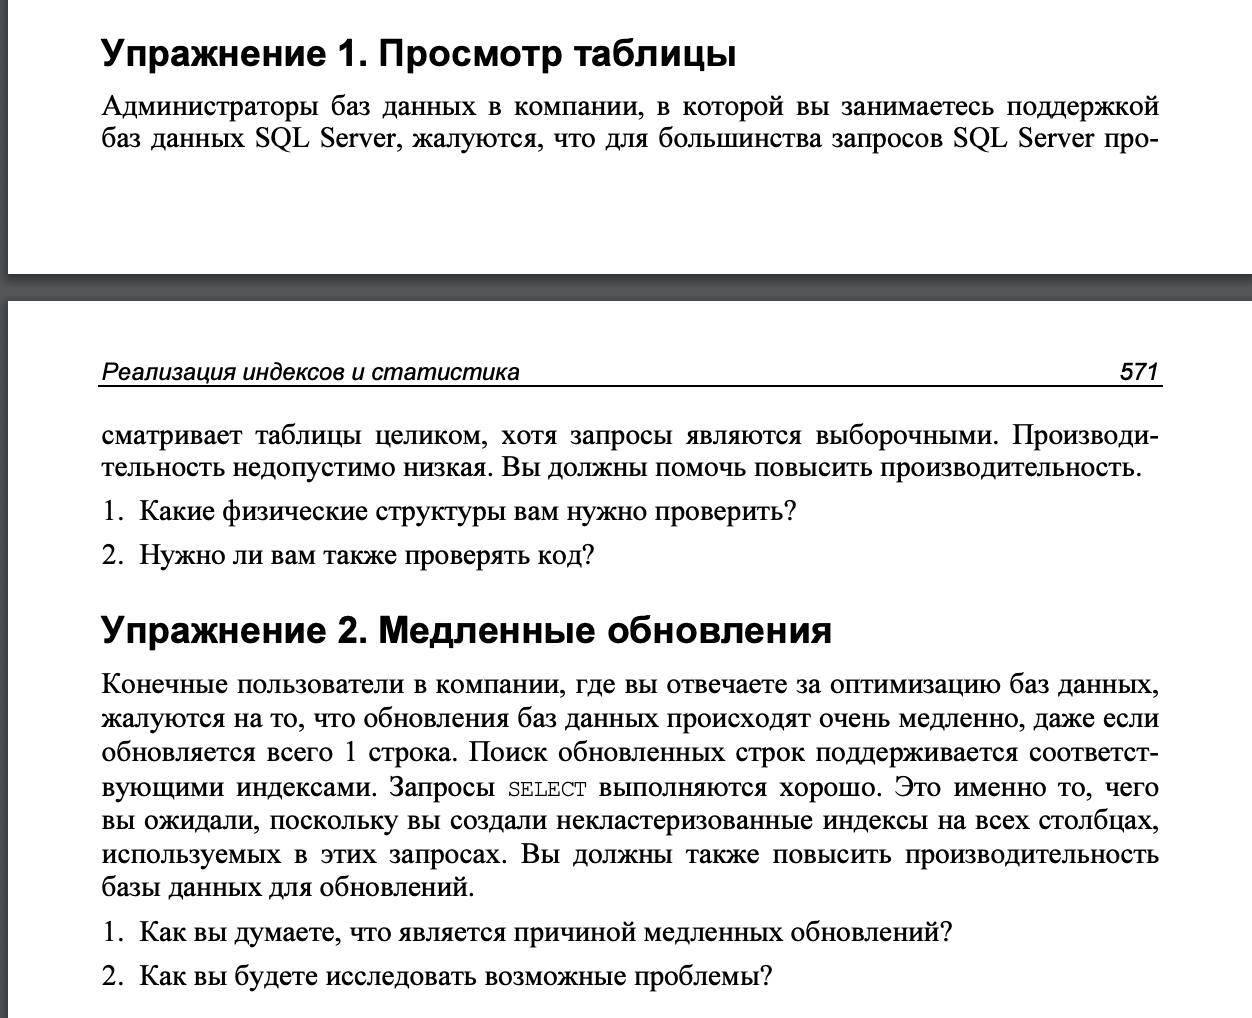
\includegraphics[width=0.8\textwidth]{img/ex19.png}
	\end{center}
	\captionsetup{justification=centering}
\end{figure}

\subsection*{Ответы}

\begin{figure}[h!]
	\begin{center}
		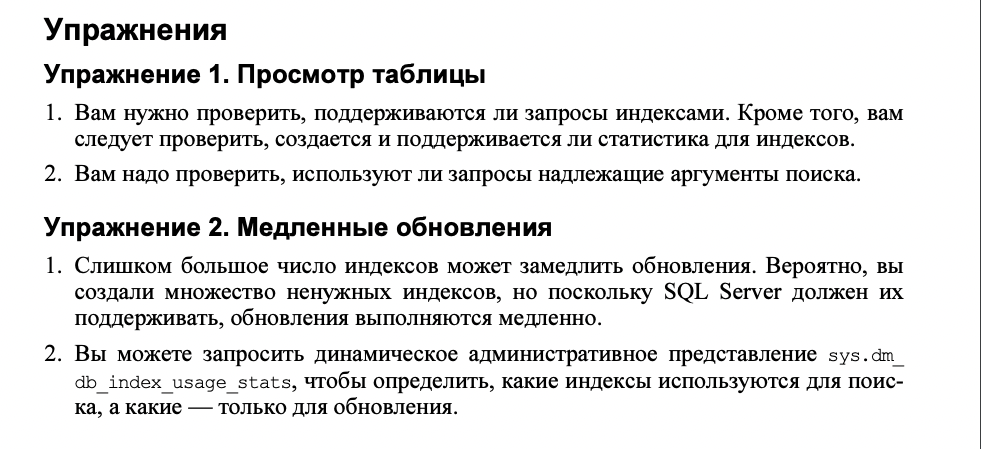
\includegraphics[width=0.8\textwidth]{img/eans19.png}
	\end{center}
	\captionsetup{justification=centering}
\end{figure}